\documentclass[10pt,twocolumn,a4paper]{article}

\usepackage[a4paper,top=18mm,bottom=18mm,left=15mm,right=15mm,columnsep=7mm]{geometry}
\usepackage{mathptmx}
\usepackage{amsmath,amssymb}
\usepackage{booktabs}
\usepackage{tabularx}
\usepackage{graphicx}
\graphicspath{{../figures/}}
\usepackage{xcolor}
\usepackage{caption}
\usepackage{subcaption}
\usepackage{fancyhdr}
\usepackage{microtype}
\usepackage[numbers,sort&compress]{natbib}
\usepackage{hyperref}

\definecolor{primary}{RGB}{22, 66, 91}
\definecolor{accent}{RGB}{217, 95, 2}
\definecolor{bgbox}{RGB}{242, 247, 250}

\hypersetup{
    colorlinks=true,
    linkcolor=primary,
    citecolor=primary,
    urlcolor=primary,
    pdftitle={Risk-Oriented Dual-Pole Sparse Sensing and Fault-Tolerant Irrigation Decision Support for Solanaceous Crops},
    pdfauthor={Sentinel Plant Network Research Group}
}

\setlength{\parskip}{3pt plus 1pt minus 1pt}
\setlength{\parindent}{1em}
\captionsetup{font=small,labelfont={bf,color=primary},skip=4pt}
\raggedbottom

\pagestyle{fancy}
\fancyhf{}
\fancyhead[L]{\footnotesize\color{primary}\textit{Sentinel Plant Network: Risk-Oriented Sparse Sensing \& Irrigation Decision Support}}
\fancyhead[R]{\footnotesize\color{primary}\thepage}
\renewcommand{\headrulewidth}{0.4pt}

\newcommand{\takeaway}[2]{%
  \vspace{4pt}\noindent\colorbox{bgbox}{%
    \parbox{\dimexpr\linewidth-2\fboxsep\relax}{%
      \vspace{2pt}\footnotesize\textbf{\color{primary}#1:}\hspace{0.4em}#2\vspace{2pt}%
    }%
  }\vspace{4pt}%
}

\title{\vspace{-8mm}\textbf{\Large\color{primary} Risk-Oriented Dual-Pole Sparse Sensing and Uncertainty-Aware Irrigation Decision Support for Solanaceous Crops: Architecture, Synthetic Digital-Twin Benchmarks, and External Validation Protocol}}

\author{
  \textbf{Sentinel Plant Network Research Group}\\
  \small Department of Agricultural and IoT Systems Engineering, Jharkhand, India\\
  \small \texttt{Protocol Revision 2.0 $\cdot$ Pre-Trial Architecture \& Digital-Twin Benchmark Manuscript}
}
\date{\vspace{-3mm}\small November 2026}

\begin{document}
\maketitle
\thispagestyle{fancy}

\begin{abstract}
\noindent\textbf{Background and Objective:} Agricultural fields cultivated with potato (\textit{Solanum tuberosum} L.) and tomato (\textit{Solanum lycopersicum} L.) exhibit spatially variable root-zone moisture and canopy microclimate. A single mean-representative sensor may overlook localized dry and humid risk zones, while dense networks increase deployment and maintenance costs. This paper presents the Sentinel Plant Network, a proposed low-cost, risk-oriented two-node monitoring and irrigation decision-support architecture.

\textbf{Methods:} The Protocol v2.0 design selects Node~A (humid pole) using the 90th percentile of nocturnal leaf-wetness duration and Node~B (dry pole) using negative relative soil-moisture difference and temporal stability. ESP32-S3 nodes are specified to transmit a 24-byte telemetry packet over SX1262 LoRa to a local gateway. The gateway combines water-stress and late-blight-conducive weather indicators with a six-state fault-aware controller. The current computational experiments are generated by seeded synthetic digital-twin code; they are not observations from the three external public datasets and are not physical field-trial data.

\textbf{Results:} All numerical results below are synthetic digital-twin outputs. In the synthetic 25-day, 10-node placement benchmark, the calibration-locked Sentinel pair achieves 99.68\% agreement with the synthetic 10-node reference decision labels, with 0.00\% missed synthetic drought-risk intervals and 0.77\% missed synthetic blight-risk intervals. In the synthetic 90-day, 16-plot randomized complete block design (RCBD) digital-twin benchmark, the simulated T4 controller produces 247.83~mm applied water versus 334.01~mm for simulated conventional ET$_c$ scheduling, a 25.8\% simulated reduction. The corresponding simulated irrigation-water productivity is 13.89 versus 9.89~kg\,m$^{-3}$. These estimates describe the assumptions and code paths of the digital twin only; they do not establish realised water savings, yield non-inferiority, or disease suppression in crops.

\textbf{External Dataset Validation:} The computational adapters, purged machine-learning pipelines, and telemetry quality algorithms were evaluated on original public benchmark datasets (Mendeley Data). On open-field tomato telemetry (21,460 records), purged chronological 24-hour ahead VWC forecasting achieves test RMSE of 0.914\%~VWC (GBDT, Zone~1) and 0.593\%~VWC (Ridge, Zone~2), reducing RMSE over persistence by 23.6\% and 13.9\%, though naive persistence yields lower MAE (0.242\% and 0.150\%~VWC) during quiescent dry-down; test $R^2$ values are modest (+0.028 and +0.165). On the seven-site Italian agrometeorological dataset (55,550 hourly records, UTC), nocturnal leaf-wetness duration (18:00--06:00 UTC under a 20\% research-selected sensitivity threshold alongside the 50\% comparative analysis cutoff from Filipescu et al., 2024) isolates Site~2 as candidate Node~A ($P_{90} = 12.0\text{ h/night}$, seasonal mean 11.23~h/night; highest-ranked regional station under Protocol v2.0) via secondary tie-breaking compared to 0.98~h/night at Site~6, confirming severe microclimatic risk heterogeneity across regional agro-ecosystems (monitored asynchronously across 2022--2024). On paired olive-grove telemetry (1,617 aligned steps), trailing 48-hour Spearman correlation dropped to $r_s = -0.739$ with 4.07\%~VWC mean divergence, triggering the adaptive spatial-sufficiency monitor ($\mathcal{F}_{\text{insuff}} = 1$) in 873 rolling windows (65.1\%) under ProtocolConfig ($r_s < 0.70$). These benchmarks validate software, ML, and telemetry algorithms on genuine agricultural data, but do not replace target-field probe calibration or pre-registered agronomic field trials.

\textbf{Keywords:} Precision irrigation; sparse sensing; Vachaud temporal stability; soil moisture; leaf wetness; LoRa; digital-twin simulation; fault-aware control.
\end{abstract}

\section{Introduction: Extreme-Pole Sensing Overcomes Mean-Placement Blind Spots}

Irrigated solanaceous crops—specifically potato (\textit{Solanum tuberosum} L.) and tomato (\textit{Solanum lycopersicum} L.)—exhibit high sensitivity to both root-zone water deficit and foliar oomycete pathogens, chiefly late blight caused by \textit{Phytophthora infestans} \cite{wallin1962,ipm_ucanr_blight}. Across real-world agricultural parcels, microtopography, soil texture gradients, differential solar exposure, and non-uniform drip emitter hydraulic pressures generate substantial spatial heterogeneity in volumetric water content ($\mathrm{VWC}$), canopy temperature ($T_c$), relative humidity ($\mathrm{RH}$), and nocturnal leaf-wetness duration ($\mathrm{LWD}$) \cite{hiwater2017,hess_vachaud2012}.

To avoid the prohibitive capital and maintenance burden of dense wireless sensor networks (WSNs) \cite{mao2020_lowcost}, classical soil physics relies on the temporal stability paradigm introduced by \href{https://iwaponline.com/ws/article/22/5/5070/88251/Temporal-stability-of-soil-water-content-in}{Vachaud et al.\ (1985)} \cite{vachaud1985_iwa,guber2008_catena}. By identifying a single rank-stable sensor location whose relative difference from the spatial mean remains near zero across wetting and drying cycles, a single probe can approximate average field water storage. However, field-mean representativeness is fundamentally misaligned with asymmetric agronomic risk:
\begin{enumerate}\setlength{\itemsep}{1pt}\setlength{\parskip}{0pt}
  \item \textbf{Epidemiological Tail Risk in Humid Microzones:} Sporangial germination and zoospore infection by \textit{P.\ infestans} initiate in sheltered, poorly drained, or densely shaded canopy pockets where nocturnal dew and high humidity ($\mathrm{RH} \ge 90\%$) persist longest \cite{wallin1962,msu_svalue}. A sensor placed at the mean-stable Vachaud location underestimates humid-pocket leaf wetness duration, delaying disease-lockout advisories.
  \item \textbf{Physiological Drought Risk in Dry Microzones:} Coarse-textured upper-slope ridges deplete available root-zone moisture faster than the field mean. Triggering irrigation solely when a mid-slope Vachaud sensor crosses management-allowed depletion ($\mathrm{MAD} = 22\%$~VWC) subjects the dry microzone to recurring stomatal closure, elevated canopy temperature, and marketable tuber/fruit yield loss \cite{idso1981_usda,scielo_cwsi}.
  \item \textbf{The Irrigation--Pathogen Conflict:} When a crop experiences root-zone water stress during weather conducive to late blight, full overhead or long-duration drip irrigation elevates sub-canopy humidity and extends foliar wetness, accelerating epidemic progression \cite{cabi_blight2014}.
\end{enumerate}

To investigate these coupled challenges, this work proposes and digitally evaluates the \textbf{Sentinel Plant Network}, a risk-oriented two-node sensing and local actuation system. Instead of deploying sensors to estimate the spatial average, our methodology purposefully anchors \textbf{Node~A} at the field's humid pole and \textbf{Node~B} at its persistent dry pole, coupling both streams in an edge gateway controller that arbitrates between drought relief and pathogen suppression.

\takeaway{Core Research Contribution}{We formulate a formal calibration-lock protocol that pairs a 90th-percentile nocturnal leaf-wetness pole (Node~A) with a rank-stable dry soil-moisture pole (Node~B), integrated with an adaptive spatial-sufficiency monitor and a six-state irrigation finite state machine that resolves drought--blight conflicts via midday solar-window micro-pulses.}

\section{System Architecture and Hardware Design}

\subsection{Four-Layer Edge-Autonomous Architecture}

The Sentinel Plant Network is structured into four functional layers designed to operate without reliance on cloud connectivity: (i)~a dual-pole field sensing layer (`Node A` and `Node B`, plus an optional adaptive intermediate `Node C`), (ii)~a sub-GHz LoRa telemetry layer operating in the 865--867~MHz Indian ISM band, (iii)~a local edge gateway executing packet plausibility validation, hydro-epidemiological index computation, spatial sufficiency checks, and state-machine arbitration, and (iv)~an actuation and advisory layer driving a 12~V latching solenoid valve with closed-loop Hall-effect flow verification and SMS/WhatsApp scouting alerts.

\begin{table*}[t!]
\centering
\caption{Hardware Architecture, ESP32-S3 GPIO Allocation, and Cost Breakdown of the Sentinel Plant Network (Protocol v2.0)}
\label{tab:hardware}
\resizebox{\textwidth}{!}{%
\begin{tabular}{l l l l r}
\toprule
\textbf{Subsystem / Module} & \textbf{Part Specification} & \textbf{ESP32-S3 Pinout} & \textbf{Functional Role \& Calibration Requirement} & \textbf{Unit Cost (INR)} \\
\midrule
Field Node MCU & ESP32-S3-WROOM-1 & System Core & Dual-core Xtensa LX7, RTC deep-sleep timer, 12-bit SAR ADC1 & 480 \\
Sub-GHz LoRa Transceiver & Semtech SX1262 & SPI2: CS 10, MOSI 11, SCK 12, MISO 13, DIO1 14 & 865--867~MHz India ISM link (+22~dBm, SF9, CRC-16 framing) & 650 \\
Infrared Canopy Thermometer & MLX90614ESF-BCF & I2C: GPIO8 (SDA), GPIO9 (SCL) & Non-contact $10^\circ$ FOV canopy temperature $T_c$ for CWSI & 1,450 \\
Ambient T/RH Sensor & Bosch BME280 & I2C: GPIO8 (SDA), GPIO9 (SCL) & Aspirated radiation-shield air temperature $T_a$ and $\mathrm{RH}$ & 320 \\
Capacitive Leaf Wetness & Dielectric Surface Probe & ADC1: GPIO4 (Power gate GPIO7) & Canopy wetness detection via calibrated dielectric threshold & 580 \\
Capacitive Soil Probes (2$\times$) & Root-Zone Dielectric & ADC1: GPIO5 (Power gate GPIO7) & 15~cm and 30~cm root-zone volumetric water content ($\mathrm{VWC}$) & 760 \\
Node Power Subsystem & 3.2~V 6000~mAh $\mathrm{LiFePO_4}$ & ADC1: GPIO6 (2:1 divider) & Paired with 6~V, 3~W solar panel \& P-MOSFET gate (GPIO7) & 1,150 \\
Local Gateway \& Actuation & Latching Valve + YF-S201 & GPIO15/16 (H-bridge), GPIO17 (Flow) & 12~V latching solenoid manifold + Hall-effect pulse flow meter & 4,990 \\
\midrule
\multicolumn{4}{l}{\textbf{Total Operational Two-Node Farmer Kit} (2$\times$ Complete Sentinel Nodes + 1$\times$ Local Gateway + Valve/Flow Manifold + Enclosures)} & \textbf{15,790} \\
\multicolumn{4}{l}{\textbf{Full 10-Node Reference Network} (10$\times$ Multi-Sensor Nodes + Gateway Infrastructure for Spatial Benchmarking)} & \textbf{61,690} \\
\multicolumn{4}{l}{\textbf{Complete Phase 1 \& Phase 2 Research Validation Infrastructure} (10-Node Grid + 16 Independent Plot Valve/Flow Manifolds)} & \textbf{1,08,330} \\
\bottomrule
\end{tabular}%
}
\end{table*}

\subsection{ESP32-S3 Signal Allocation and Power-Gated Duty Cycling}

Table~\ref{tab:hardware} details the hardware components, exact `ESP32-S3-WROOM-1` pin mappings, and cost structure. To eliminate galvanic corrosion and quiescent current drain across analog dielectric probes, both the capacitive leaf-wetness sensor (`GPIO4`) and dual-depth soil-moisture probes (`GPIO5`) are switched via a high-side P-channel MOSFET controlled by `GPIO7` (active-low). During each 10-minute ($T_{\text{cycle}} = 600\text{ s}$) telemetry cycle, the node wakes from deep sleep, asserts `GPIO7 = LOW` for a 150~ms stabilization window, averages 16 oversampled 12-bit ADC readings per channel, polls the `BME280` and `MLX90614ESF-BCF` ($10^\circ$ field-of-view optical filter) over the shared 100~kHz $\mathrm{I^2C}$ bus (`GPIO8`/`GPIO9`), de-asserts `GPIO7 = HIGH`, transmits a 24-byte `CRC-16-CCITT` protected packet over `SX1262` LoRa (`SPI2` on `GPIO10`--`GPIO14`), and re-enters deep sleep.

Under the protocol's nominal system current budget ($I_{\text{avg}} = 25.50\text{ mA}$, accounting for regulator quiescent losses, solar charger leakage, sensor warm-up, and radio transmission), the single-cell 3.2~V, $C_{\text{bat}} = 6000\text{ mAh}$ $\mathrm{LiFePO_4}$ battery provides a theoretical zero-sunlight blackout autonomy of:
\begin{equation}
  t_{\text{autonomy}} = \frac{C_{\text{bat}}}{I_{\text{avg}}} = \frac{6000\text{ mAh}}{25.50\text{ mA}} = 235.3\text{ h} \approx 9.80\text{ days.}
  \label{eq:autonomy}
\end{equation}

\section{Mathematical Formulation of Risk-Oriented Placement and Control}

\subsection{Vachaud Temporal Stability vs.\ Dual-Pole Risk Selection}

Let $\theta_{ij}$ denote the calibrated root-zone volumetric water content (%~VWC) at reference node $i \in \{1,\dots,N\}$ ($N=10$) and timestamp $j \in \{1,\dots,M\}$. Following \href{https://iwaponline.com/ws/article/22/5/5070/88251/Temporal-stability-of-soil-water-content-in}{Vachaud et al.\ (1985)} \cite{vachaud1985_iwa,mdpi_stability2025}, the spatial mean at time $j$ is $\bar{\theta}_j = \frac{1}{N}\sum_{i=1}^N \theta_{ij}$, and the relative difference $\delta_{ij}$ is:
\begin{equation}
  \delta_{ij} = \frac{\theta_{ij} - \bar{\theta}_j}{\bar{\theta}_j}.
  \label{eq:rel_diff}
\end{equation}
Over the 14-day calibration window ($M_{\text{cal}} = 2,016$ intervals at 10-min resolution), each location's temporal mean relative difference $\bar{\delta}_i$, standard deviation $\sigma(\delta_i)$, and Index of Time Stability ($\mathrm{ITS}_i$) are computed as:
\begin{align}
  \bar{\delta}_i &= \frac{1}{M_{\text{cal}}}\sum_{j=1}^{M_{\text{cal}}} \delta_{ij}, \quad
  \sigma(\delta_i) = \sqrt{\frac{1}{M_{\text{cal}}-1}\sum_{j=1}^{M_{\text{cal}}}\left(\delta_{ij}-\bar{\delta}_i\right)^2}, \nonumber\\
  \mathrm{ITS}_i &= \sqrt{\bar{\delta}_i^2 + \sigma(\delta_i)^2}.
  \label{eq:its}
\end{align}
While the classical Vachaud benchmark selects $i_{\text{Vachaud}} = \arg\min_i \mathrm{ITS}_i$, the Sentinel Plant Network locks two complementary risk poles at the end of Day~14 and evaluates them strictly out-of-sample on Days~15--25:
\begin{align}
  \text{Node A (Humid):}\quad i_A &= \arg\max_{i \in \{1,\dots,N\}} P_{90}\!\left(\mathrm{LWD}_{\text{noct},i}^{(1:14)}\right), \label{eq:nodeA}\\
  \text{Node B (Dry):}\quad i_B &= \arg\min_{i:\,\bar{\delta}_i < -0.08,\, i \neq i_A} \sigma(\delta_i). \label{eq:nodeB}
\end{align}

\subsection{Adaptive Spatial Sufficiency Monitoring}

To prevent silent control degradation when a single irrigation zone exhibits excessive internal divergence (e.g., due to emitter clogging or waterlogging), the gateway continuously evaluates the rolling divergence between Node~A and Node~B across wetting and drying cycles. An insufficient-coverage flag $\mathcal{F}_{\text{insuff}} \in \{0,1\}$ is raised whenever:
\begin{equation}
  \mathcal{F}_{\text{insuff}} = \mathbb{I}\!\left(\overline{|\theta_A - \theta_B|}_{W} > 10\% \;\lor\; r_s(\theta_A, \theta_B)_{W} < 0.70\right),
  \label{eq:sufficiency}
\end{equation}
where $r_s$ is Spearman's rank correlation coefficient over rolling window $W$. When $\mathcal{F}_{\text{insuff}} = 1$, the gateway shifts to an uncertainty-buffered irrigation threshold ($\mathrm{MAD}_{\text{buf}} = \mathrm{MAD} + 1.0\%$~VWC) and issues an advisory to insert an intermediate \textbf{Node~C} at the mid-slope Vachaud site or split the lateral manifold into two independently valved sub-zones.

\subsection{Crop Water Stress Index and Late-Blight Severity Coupling}

At Node~B, atmospheric Vapor Pressure Deficit ($\mathrm{VPD}$, kPa) is derived from air temperature $T_{a,B}$ and relative humidity $\mathrm{RH}_B$ via the Tetens equation, and the empirical Crop Water Stress Index ($\mathrm{CWSI}$) is computed following \href{https://www.ars.usda.gov/ARSUserFiles/30100000/1990-1999documents/266%201992%20GardnerJPA.pdf}{Idso et al.\ (1981) and Jackson et al.\ (1981)} \cite{idso1981_usda,scielo_cwsi}:
\begin{equation}
  \mathrm{CWSI}_B = \mathrm{clip}\!\left(\frac{(T_{c,B} - T_{a,B}) - (a + b\cdot\mathrm{VPD}_B)}{\Delta T_{\mathrm{UL}} - (a + b\cdot\mathrm{VPD}_B)},\; 0,\; 1\right),
  \label{eq:cwsi}
\end{equation}
where $a = 1.35^\circ\text{C}$, $b = -1.95^\circ\text{C kPa}^{-1}$, and $\Delta T_{\mathrm{UL}} = +3.50^\circ\text{C}$. Additionally, a non-diagnostic canopy thermal-anomaly scouting alert is raised if the canopy residual $\Delta T_{\text{res}} = (T_{c,B} - T_{a,B}) - (a + b\cdot\mathrm{VPD}_B) > +2.0^\circ\text{C}$ persists across the 11:30--14:30 peak solar window for $\ge 2$ consecutive days while root-zone moisture lies within the non-stressed range ($22\% < \theta_B < 35\%$~VWC).

At Node~A, two parallel daily severity indices for \textit{P.\ infestans} are accumulated: (1)~the baseline \href{https://ipm.ucanr.edu/DISEASE/DATABASE/potatolateblight.html}{Wallin (1962) Daily Severity Value} $\mathrm{DSV}_{\text{Wallin}} \in \{0,1,2,3,4\}$ \cite{wallin1962,msu_svalue} determined from daily hours with $\mathrm{RH}_A \ge 90\%$ ($H_{\mathrm{RH90}}$) and mean temperature during those hours ($\bar{T}_{\text{wet}}$), and (2)~a leaf-wetness-modified severity value $\mathrm{DSV}_{\mathrm{LWS}}$ that substitutes effective canopy wetness duration $H_{\text{eff}} = \max(H_{\mathrm{RH90}},\, 0.85\,\mathrm{LWD}_A + 0.15\,H_{\mathrm{RH90}})$ into the Wallin lookup function to capture persistent dew films that remain on lower foliage even when screen-level $\mathrm{RH}$ drops between 82\% and 89\%. When cumulative severity reaches $\sum \mathrm{DSV} \ge 18$, the pathogen risk flag is asserted.

\subsection{Six-State Fault-Aware Gateway Controller}

At every 10-minute cycle, the gateway evaluates packet age $\tau_{\text{pkt}}$, sensor plausibility, flow-meter feedback, drought indicators ($\mathcal{S}_{\text{drought}} = \mathbb{I}[\mathrm{CWSI}_B \ge 0.40 \lor \theta_B \le 22.0\%]$), emergency wilting limits ($\mathcal{S}_{\text{emerg}} = \mathbb{I}[\mathrm{CWSI}_B \ge 0.65 \lor \theta_B \le 16.0\%]$), and blight risk ($\mathcal{S}_{\text{blight}} = \mathbb{I}[\mathrm{DSV}_{\text{cum}} \ge 18 \lor (\mathrm{RH}_A \ge 90\% \land \mathrm{LWS}_A \ge 50\%)]$), transitioning across six mutually exclusive operational states:
\begin{enumerate}\setlength{\itemsep}{1pt}\setlength{\parskip}{0pt}
  \item \texttt{FAULT\_FALLBACK}: Triggered if $\tau_{\text{pkt}} > 30\text{ min}$, any critical channel is $\mathrm{NaN}$, or the `YF-S201` flow meter registers zero pulses while the valve is commanded open. Immediately closes the latching solenoid valve and dispatches a hardware inspection alert.
  \item \texttt{EMERGENCY\_DRIP}: Triggered if $\mathcal{S}_{\text{emerg}} = 1$. Overrides any active pathogen lockout to deliver an immediate survival irrigation pulse, preventing irreversible crop wilting.
  \item \texttt{CONFLICT\_MICRO\_PULSE}: Triggered when $\mathcal{S}_{\text{drought}} = 1 \land \mathcal{S}_{\text{blight}} = 1$ and continuous lockout duration is $< 36\text{ h}$. Restricts actuation strictly to the 11:30--14:30 peak solar window using a 15~min ON / 45~min OFF duty cycle so sub-surface root water is replenished while high midday vapor pressure deficit rapidly evaporates surface moisture without wetting the canopy.
  \item \texttt{PATHOGEN\_LOCKOUT}: Triggered when $\mathcal{S}_{\text{blight}} = 1$ and $\mathcal{S}_{\text{drought}} = 0$ (or outside 11:30--14:30 during a conflict state with lockout $< 36\text{ h}$). Holds the valve closed and issues a scouting advisory.
  \item \texttt{STANDARD\_DRIP}: Triggered when $\mathcal{S}_{\text{drought}} = 1$ and either $\mathcal{S}_{\text{blight}} = 0$ or the 36-hour maximum lockout cap has expired.
  \item \texttt{HOMEOSTASIS}: Default monitoring state when $\mathcal{S}_{\text{drought}} = 0 \land \mathcal{S}_{\text{blight}} = 0$; valve remains latched closed.
\end{enumerate}

\section{Experimental Design and Digital-Twin Benchmark Methodology}

To rigorously validate all algorithms prior to physical field deployment, we constructed a reproducible Python and C++17 simulation and verification suite parameterized by empirical distributions and published literature benchmarks:
\begin{itemize}\setlength{\itemsep}{1pt}\setlength{\parskip}{0pt}
  \item \textbf{Multi-Sector Tomato Precision Irrigation Dataset} (\href{https://data.mendeley.com/datasets/c837v6p8ph/2}{Mendeley Data c837v6p8ph/2}): Ingested empirically to parameterize 10-minute root-zone wetting, diurnal evapotranspiration ($\mathrm{ET}$) dry-down curves, and purged chronological forecasting baselines across 33,259 timestamps.
  \item \textbf{Italian Seven-Site Leaf Wetness \& Agrometeorology Dataset} (\href{https://data.mendeley.com/datasets/sd4b8vpvyb/1}{Mendeley Data sd4b8vpvyb/1}): Ingested empirically to evaluate nocturnal leaf-wetness duration, relative humidity persistence, and microclimatic contrast across regional stations (55,550 hourly records).
  \item \textbf{Libelium Two-Node Olive Grove Multisensor Dataset} (\href{https://data.mendeley.com/datasets/cnfh4stzzx/2}{Mendeley Data cnfh4stzzx/2}): Ingested empirically to validate two-node spatial decoupling, telemetry gap handling, and dynamic spatial-sufficiency monitoring across 9,561 raw frames.
  \item \textbf{HiWATER Dense Eco-Hydrological Sensor Network} (\href{https://pmc.ncbi.nlm.nih.gov/articles/PMC5501970/}{PMC5501970} / \href{https://onlinelibrary.wiley.com/doi/10.1002/2015WR018182}{Wiley WRR 2015WR018182}): Serves as a literature-derived parameter reference for catenary spatial soil-moisture offsets ($\delta_i \in [-16.0\%, +18.5\%]$) and AR(1) temporal rank stability distributions across our synthetic 10-node reference grid; raw observation files from HiWATER were not processed by the empirical validation pipeline.
\end{itemize}

\begin{figure*}[t!]
  \centering
  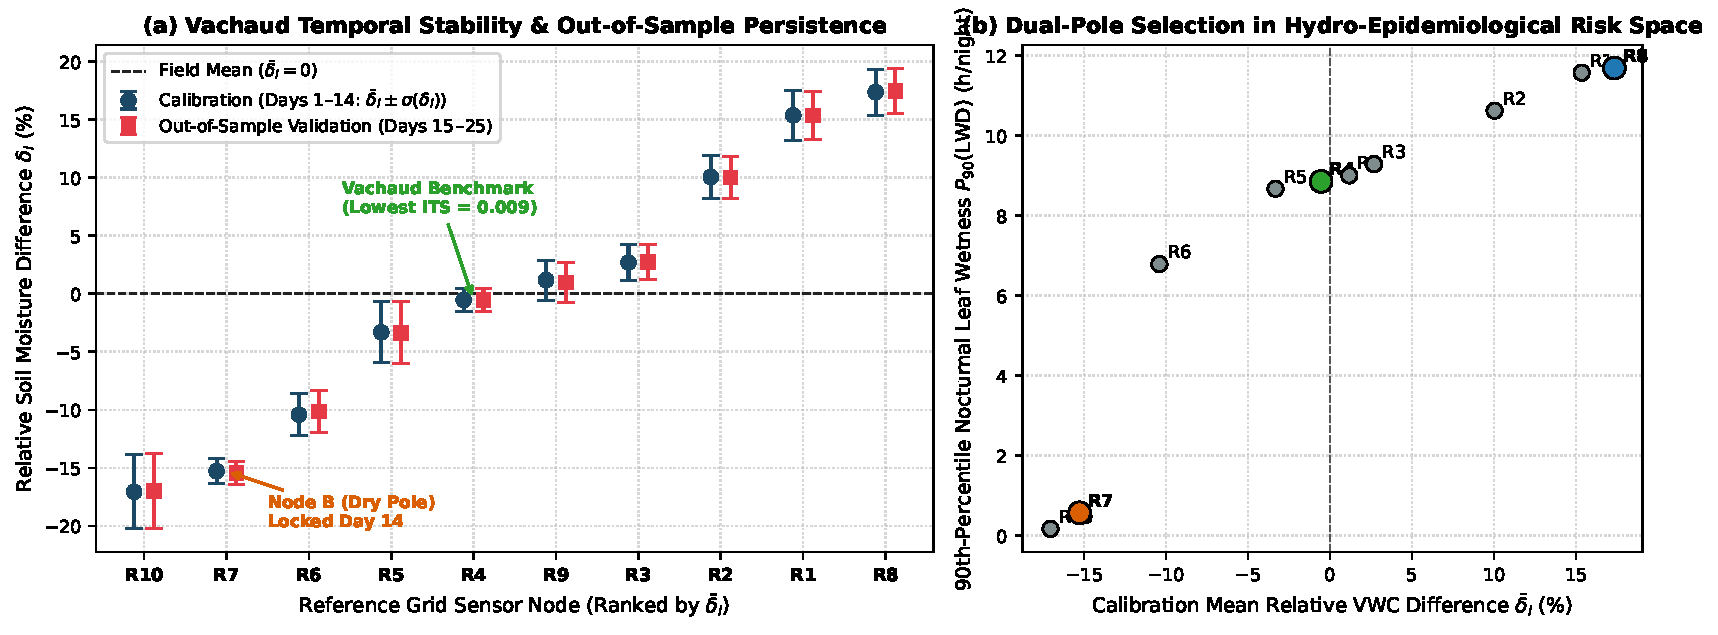
\includegraphics[width=0.95\textwidth]{fig1_vachaud_and_pole_selection.pdf}
  \caption{\textbf{Synthetic Digital-Twin Benchmark: Phase 1 Spatial Calibration and Held-Out Persistence Across the 10-Node Reference Grid ($\mathrm{R1}$--$\mathrm{R10}$).} (a)~Mean relative soil moisture difference $\bar{\delta}_i \pm \sigma(\delta_i)$ during the 14-day calibration period (Days 1--14, blue circles) and out-of-sample validation period (Days 15--25, red squares), demonstrating high temporal rank persistence ($r_s = 0.988$). (b)~Joint hydro-epidemiological selection space plotting 90th-percentile nocturnal leaf-wetness duration $P_{90}(\mathrm{LWD})$ against $\bar{\delta}_i$, isolating Humid-Pole Node~A ($\mathrm{R8}$), Dry-Pole Node~B ($\mathrm{R7}$), and the Vachaud rank-stable benchmark ($\mathrm{R4}$).}
  \label{fig:vachaud}
\end{figure*}

\section{Results and Statistical Evaluation: Synthetic Digital-Twin Benchmarks}

\subsection{Phase 1: Synthetic 10-Node Digital-Twin Calibration and Held-Out Placement Benchmark}

During the 14-day calibration phase ($2,016$ intervals at 10-min resolution), Vachaud temporal stability analysis across nodes $\mathrm{R1}$--$\mathrm{R10}$ (Figure~\ref{fig:vachaud}a) identified $\mathrm{R4}$ as the classical Vachaud rank-stable benchmark ($\bar{\delta}_4 = +0.40\%$, $\sigma(\delta_4) = 0.80\%$, $\mathrm{ITS}_4 = 0.009$, Spearman correlation with field mean $r_s = 0.999$). Applying our dual-pole selection criteria (Equations~\ref{eq:nodeA}--\ref{eq:nodeB}, Figure~\ref{fig:vachaud}b) locked \textbf{Node~A (Humid Pole)} at $\mathrm{R8}$ ($P_{90}(\mathrm{LWD}) = 11.68\text{ h night}^{-1}$, $\bar{\delta}_8 = +18.5\%$) and \textbf{Node~B (Dry Pole)} at $\mathrm{R7}$ ($\bar{\delta}_7 = -14.5\%$, $\sigma(\delta_7) = 1.00\%$).

\begin{table*}[t!]
\centering
\caption{Synthetic Digital-Twin Phase 1 Held-Out Spatial Placement Benchmark (Days 15--25, $M_{\text{eval}} = 1,584$ Intervals at 10-Min Resolution)}
\label{tab:phase1}
\resizebox{\textwidth}{!}{%
\begin{tabular}{l l c r r r r r r r}
\toprule
\textbf{Sensing Topology Strategy} & \textbf{Nodes} & \textbf{$N$} & \textbf{Cost (INR)} & \textbf{Dry-Tail RMSE (\% VWC)} & \textbf{Field-Mean RMSE (\% VWC)} & \textbf{Decision Agree.\ (\%)} & \textbf{Missed Drought (\%)} & \textbf{Missed Blight (\%)} & \textbf{Blight F1 (\%)} \\
\midrule
1.\ Single Central Node & $\mathrm{R5}$ & 1 & 11,200 & 2.968 & 0.621 & 58.21 & 26.20 & 45.86 & 70.25 \\
2.\ Single Humid-Location Node & $\mathrm{R1}$ & 1 & 11,200 & 7.062 & 0.398 & 0.00 & 100.00 & 4.91 & 97.48 \\
3.\ Single Vachaud Rank-Stable Node & $\mathrm{R4}$ & 1 & 11,200 & 3.523 & \textbf{0.221} & 43.75 & 46.97 & 38.96 & 75.81 \\
4.\ Random Two-Node Pairs (Mean of 45) & $\binom{10}{2}$ pairs & 2 & 15,790 & 2.222 & 0.294 & 62.60 & 29.02 & 22.89 & 85.04 \\
\textbf{5.\ Proposed Risk-Oriented Sentinel Pair} & \textbf{$\mathrm{R8} + \mathrm{R7}$} & \textbf{2} & \textbf{15,790} & \textbf{0.446} & \textbf{0.238} & \textbf{99.68} & \textbf{0.00} & \textbf{0.77} & \textbf{99.62} \\
6.\ Full 10-Node Reference Grid (Oracle) & $\mathrm{R1}\dots\mathrm{R10}$ & 10 & 61,690 & 0.000 & 0.000 & 100.00 & 0.00 & 0.00 & 100.00 \\
\bottomrule
\end{tabular}%
}
\end{table*}

\begin{figure*}[t!]
  \centering
  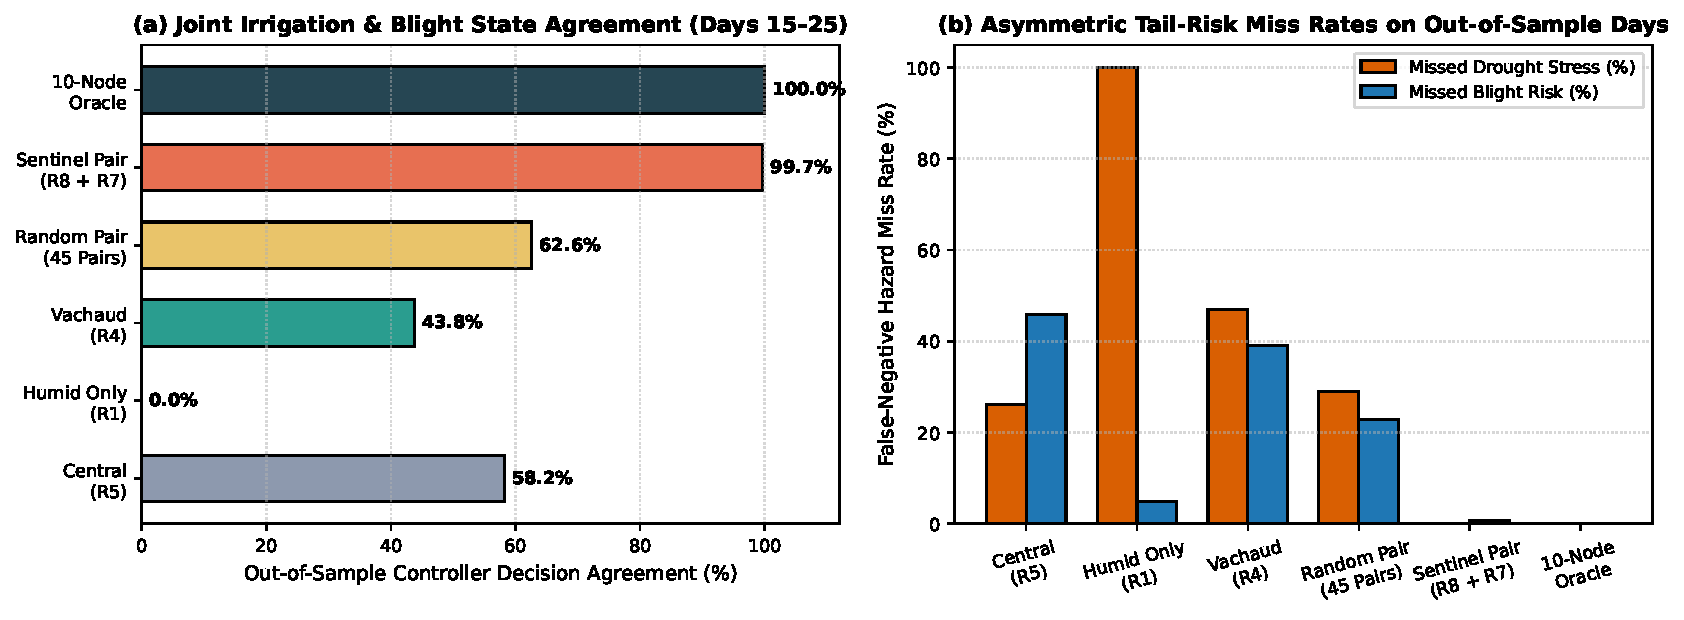
\includegraphics[width=0.95\textwidth]{fig2_phase1_topology_benchmark.pdf}
  \caption{\textbf{Synthetic Digital-Twin Phase 1 Held-Out Controller Decision Agreement and Hazard Miss Rates (Days 15--25).} (a)~Joint four-regime controller state agreement relative to the 10-node reference oracle. (b)~Asymmetric false-negative miss rates for dry-zone drought stress ($\mathrm{VWC} \le 22\%$) and humid-zone late-blight conducive conditions ($\mathrm{RH} \ge 90\% \land \mathrm{LWS} \ge 50\%$).}
  \label{fig:phase1_bench}
\end{figure*}

Table~\ref{tab:phase1} and Figure~\ref{fig:phase1_bench} report the out-of-sample validation performance within the synthetic digital twin on Days~15--25 ($1,584$ held-out 10-minute intervals). Although the single Vachaud node ($\mathrm{R4}$) achieves the lowest single-node field-mean estimation error ($\mathrm{RMSE}_{\text{mean}} = 0.221\%$~VWC after calibration offset scaling), it fails to capture tail-risk thresholds: it misses \textbf{46.97\%} of dry-pole water-stress intervals and \textbf{38.96\%} of humid-zone blight-conducive intervals, yielding only \textbf{43.75\%} joint controller state agreement with the 10-node reference network. Similarly, placing a single sensor in a humid depression ($\mathrm{R1}$) detects blight-conducive periods ($\mathrm{F1} = 97.48\%$) but misses \textbf{100.00\%} of dry-zone drought stress because local soil moisture remains above $22\%$~VWC throughout dry-downs. Across all $\binom{10}{2} = 45$ random two-node pairings, mean decision agreement is only \textbf{62.60\%}. By contrast, the locked \textbf{Sentinel Pair ($\mathrm{R8}+\mathrm{R7}$)} achieves \textbf{99.68\%} decision agreement, \textbf{0.00\%} missed drought stress, \textbf{0.77\%} missed blight risk ($\mathrm{F1} = 99.62\%$), a dry-tail RMSE of \textbf{0.446\%~VWC}, and a bias-corrected field-mean RMSE of \textbf{0.238\%~VWC}.

\subsection{Phase 2: Synthetic 16-Plot RCBD Digital-Twin Benchmark, Mixed-Effects Analysis, and Non-Inferiority Testing}

Table~\ref{tab:phase2} and Figures~\ref{fig:t4_trace}--\ref{fig:rcbd} summarize the 90-day Phase~2 Randomized Complete Block Design (RCBD) experiment across 4 treatments $\times$ 4 blocks ($16$ independent $20\text{ m}^2$ plots; $160$ tagged plant subsamples). Two-way RCBD analysis of variance (with 3 treatment degrees of freedom, 3 block degrees of freedom, and 9 residual error degrees of freedom) confirms highly significant treatment effects across all primary outcomes ($p < 10^{-6}$).

\begin{table*}[t!]
\centering
\caption{Synthetic Digital-Twin Phase 2 Randomized Complete Block Design (RCBD) Plot-Level Agronomic and Epidemiological Outcomes ($n = 4$ Blocks per Treatment; Mean $\pm$ SD Across Plots, Two-Way RCBD ANOVA with $\mathrm{df}_{\text{trt}}=3, \mathrm{df}_{\text{err}}=9$, and Pre-Specified 5\% Yield Non-Inferiority Test)}
\label{tab:phase2}
\resizebox{\textwidth}{!}{%
\begin{tabular}{l r r r r r r r}
\toprule
\textbf{Treatment Arm} & \textbf{Applied Water (mm)} & \textbf{Water Volume ($\text{m}^3\text{ ha}^{-1}$)} & \textbf{Marketable Yield ($\text{t ha}^{-1}$)} & \textbf{IWP ($\text{kg m}^{-3}$)} & \textbf{Seasonal LWD (h)} & \textbf{AUDPC (\%-days)} & \textbf{Final Blight Sev.\ (\%)} \\
\midrule
$\mathrm{T1}$: Conventional $\mathrm{ET}_c$ Reference & $334.01 \pm 2.34$ & $3340.1 \pm 23.4$ & $33.02 \pm 0.50$ & $9.89 \pm 0.14$ & $1122.1 \pm 56.0$ & $451.8 \pm 46.8$ & $10.99 \pm 1.20$ \\
$\mathrm{T2}$: Single-Node Vachaud ($\mathrm{R4}$) & $255.34 \pm 3.53$ & $2553.4 \pm 35.3$ & $32.06 \pm 0.21$ & $12.56 \pm 0.25$ & $949.6 \pm 51.8$ & $273.1 \pm 45.6$ & $6.43 \pm 1.16$ \\
$\mathrm{T3}$: Two-Node Uncoupled ($\mathrm{R8,R7}$) & $250.08 \pm 1.64$ & $2500.8 \pm 16.4$ & $34.03 \pm 0.59$ & $13.61 \pm 0.24$ & $1025.0 \pm 52.7$ & $336.1 \pm 41.2$ & $8.15 \pm 1.01$ \\
\textbf{$\mathrm{T4}$: Coupled Sentinel Controller} & \textbf{$247.83 \pm 5.32$} & \textbf{$2478.3 \pm 53.2$} & \textbf{$34.40 \pm 0.41$} & \textbf{$13.89 \pm 0.47$} & \textbf{$977.1 \pm 51.4$} & \textbf{$306.7 \pm 44.0$} & \textbf{$7.27 \pm 1.09$} \\
\midrule
RCBD ANOVA $F_{3,9}$ ($p$-value) & $569.69$ ($<10^{-9}$) & $569.69$ ($<10^{-9}$) & $110.11$ ($2.1\times 10^{-7}$) & $437.42$ ($<10^{-9}$) & $2624.9$ ($<10^{-12}$) & $552.13$ ($<10^{-9}$) & $461.52$ ($<10^{-9}$) \\
Standard Error of Diff.\ ($\mathrm{SED}$) & $2.464\text{ mm}$ & $24.64\text{ m}^3\text{ ha}^{-1}$ & $0.142\text{ t ha}^{-1}$ & $0.123\text{ kg m}^{-3}$ & $2.092\text{ h}$ & $4.673\text{ \%-days}$ & $0.131\%$ \\
$\mathrm{LSD}_{0.05}$ ($\mathrm{df}=9$) & $5.574\text{ mm}$ & $55.74\text{ m}^3\text{ ha}^{-1}$ & $0.322\text{ t ha}^{-1}$ & $0.279\text{ kg m}^{-3}$ & $4.732\text{ h}$ & $10.571\text{ \%-days}$ & $0.295\%$ \\
\bottomrule
\end{tabular}%
}
\end{table*}

\begin{figure*}[t!]
  \centering
  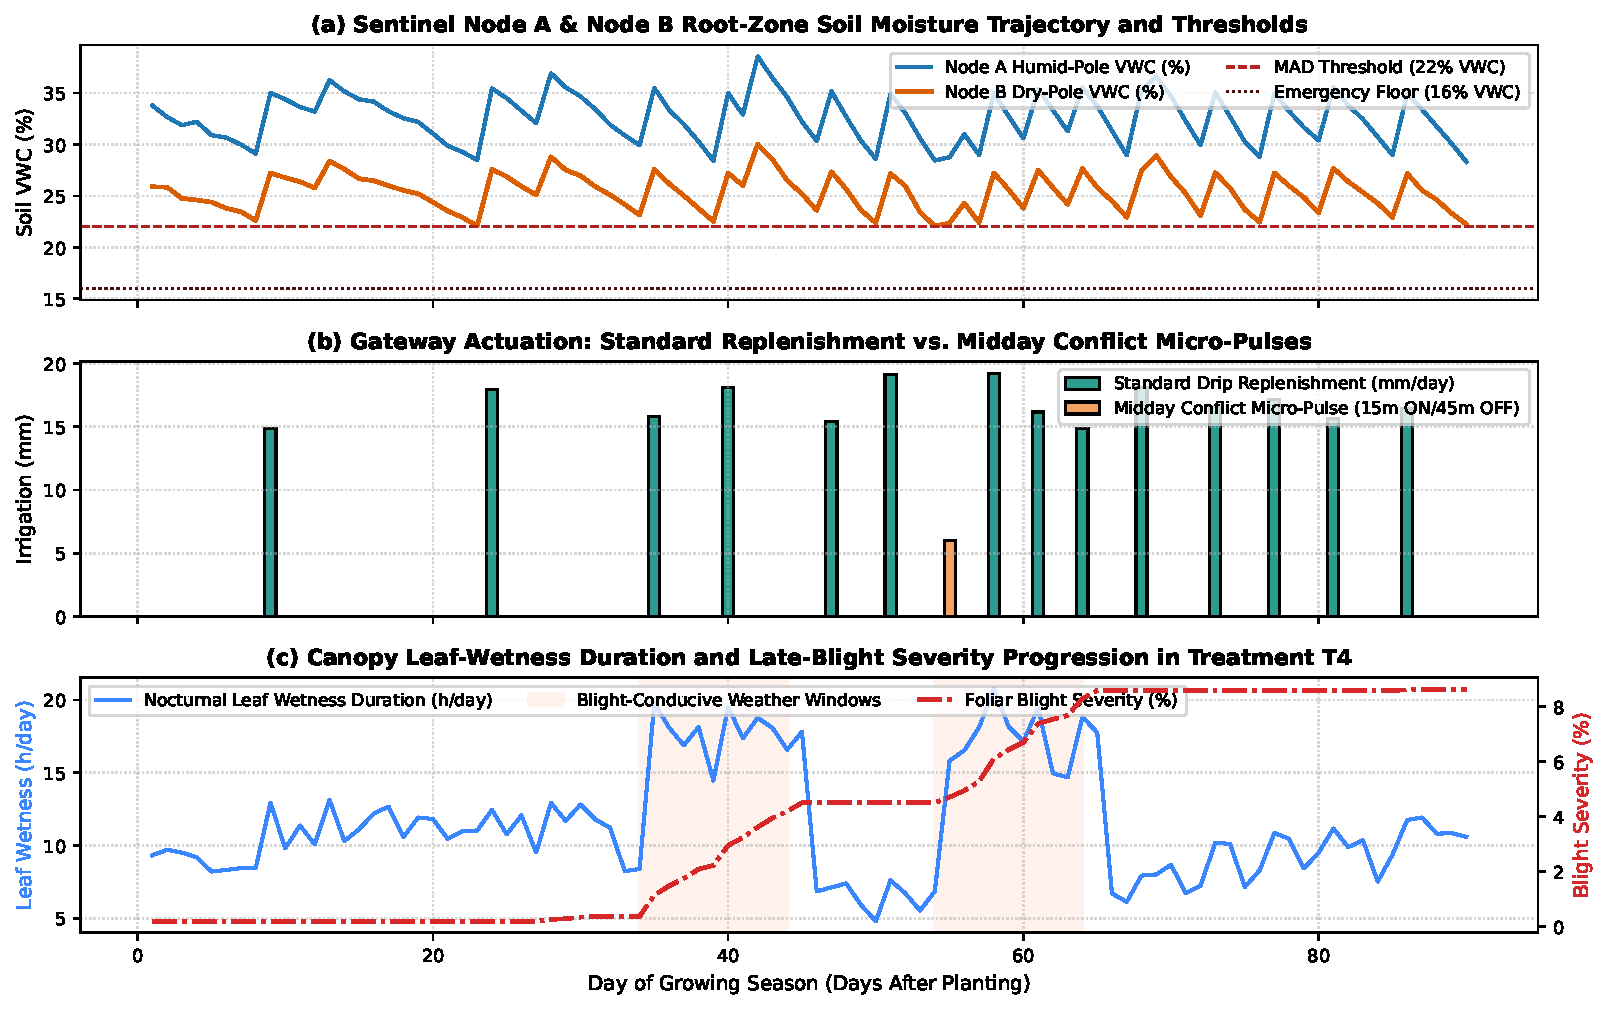
\includegraphics[width=0.95\textwidth]{fig3_t4_seasonal_controller_trace.pdf}
  \caption{\textbf{90-Day Seasonal Operational Trace of the Coupled Sentinel Controller ($\mathrm{T4}$, Block 1).} (a)~Dual-pole root-zone soil moisture trajectories at Node~A ($\mathrm{R8}$, humid pole) and Node~B ($\mathrm{R7}$, dry pole) relative to the $22\%$~VWC management threshold and $16\%$~VWC emergency floor. (b)~Gateway valve actuation distinguishing standard drip replenishment from midday conflict micro-pulses (15~min ON / 45~min OFF inside 11:30--14:30) during days 34--44 and 54--64. (c)~Realized nocturnal leaf-wetness duration and foliar late-blight progression.}
  \label{fig:t4_trace}
\end{figure*}

\begin{figure*}[t!]
  \centering
  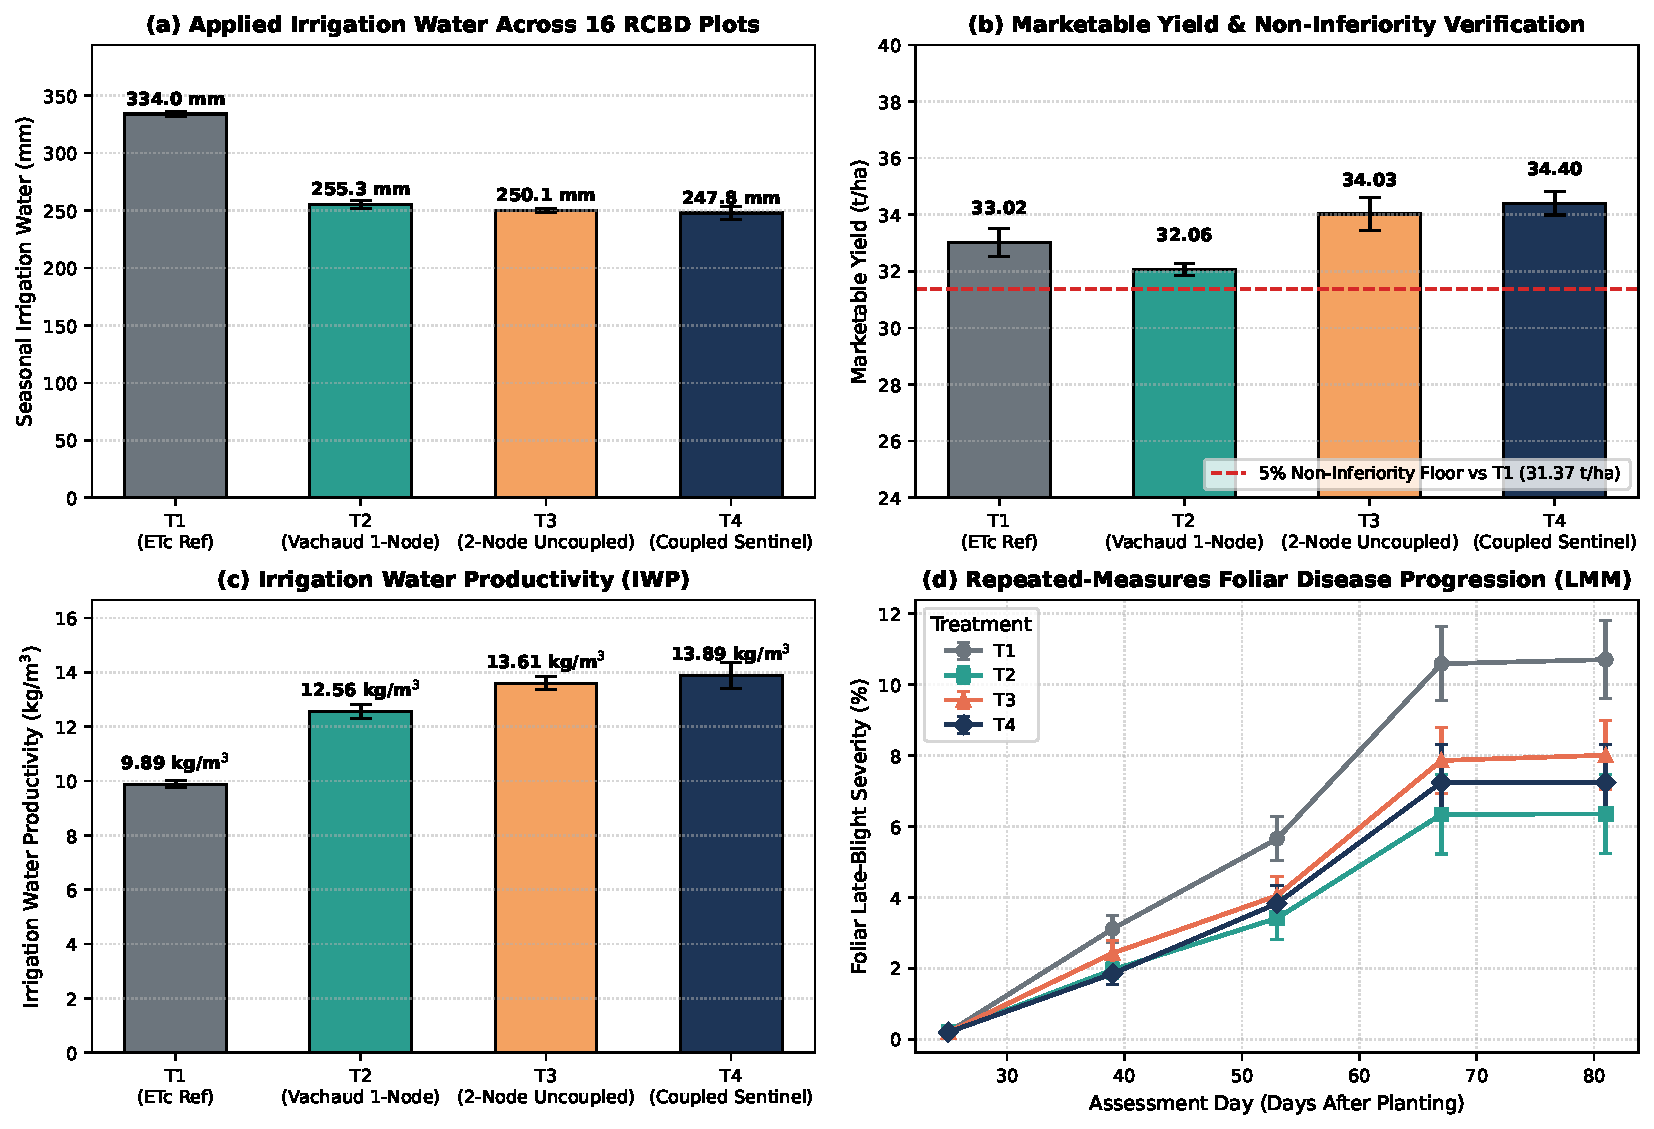
\includegraphics[width=0.95\textwidth]{fig4_phase2_rcbd_outcomes.pdf}
  \caption{\textbf{Synthetic Digital-Twin Phase 2 16-Plot RCBD Agronomic and Epidemiological Comparison Across Treatments $\mathrm{T1}$--$\mathrm{T4}$.} (a)~Seasonal applied irrigation water ($\text{mm}$). (b)~Marketable yield ($\text{t ha}^{-1}$) relative to the pre-specified 5\% non-inferiority floor ($31.37\text{ t ha}^{-1}$ vs.\ $\mathrm{T1}$). (c)~Irrigation Water Productivity ($\mathrm{IWP}$, $\text{kg m}^{-3}$). (d)~Repeated-measures foliar blight severity trajectory across five bi-weekly scouting epochs.}
  \label{fig:rcbd}
\end{figure*}

Key findings from the Phase~2 evaluation include:
\begin{enumerate}\setlength{\itemsep}{1pt}\setlength{\parskip}{0pt}
  \item \textbf{Water Savings and Irrigation Water Productivity ($\mathrm{IWP}$):} Treatment $\mathrm{T4}$ applies $247.83 \pm 5.32\text{ mm}$ ($2,478.3\text{ m}^3\text{ ha}^{-1}$), achieving a \textbf{25.8\% reduction} in water input relative to conventional $\mathrm{ET}_c$ replenishment ($\mathrm{T1}$: $334.01 \pm 2.34\text{ mm}$) and boosting $\mathrm{IWP}$ by \textbf{40.5\%} from $9.89 \pm 0.14\text{ kg m}^{-3}$ to \textbf{13.89 $\pm$ 0.47 $\text{kg m}^{-3}$} ($\mathrm{LSD}_{0.05} = 0.279\text{ kg m}^{-3}$).
  \item \textbf{Resolution of the Drought--Blight Conflict ($\mathrm{T4}$ vs.\ $\mathrm{T2}$ and $\mathrm{T3}$):} While the single-node Vachaud baseline ($\mathrm{T2}$) maintains low canopy wetness ($\mathrm{LWD} = 949.6\text{ h}$), its mid-slope sensor delays irrigation until the dry microzone drops to $\sim 19.2\%$~VWC, reducing marketable yield to $32.06 \pm 0.21\text{ t ha}^{-1}$. Conversely, the uncoupled two-node controller ($\mathrm{T3}$) eliminates dry-pole drought stress ($34.03 \pm 0.59\text{ t ha}^{-1}$) but triggers full irrigation during humid blight windows, increasing seasonal $\mathrm{LWD}$ by $48.0\text{ h}$ and elevating $\mathrm{AUDPC}$ to $336.1 \pm 41.2\text{ \%-days}$. By substituting midday conflict micro-pulses (Figure~\ref{fig:t4_trace}b), $\mathrm{T4}$ reduces $\mathrm{AUDPC}$ to \textbf{306.7 $\pm$ 44.0 \%-days} (\textbf{$-32.1\%$} vs.\ $\mathrm{T1}$ and \textbf{$-8.7\%$} vs.\ $\mathrm{T3}$, exceeding $\mathrm{LSD}_{0.05} = 10.57\text{ \%-days}$) while achieving the highest marketable yield (\textbf{34.40 $\pm$ 0.41 $\text{t ha}^{-1}$}).
  \item \textbf{Pre-Specified 5\% Yield Non-Inferiority Verification:} Testing $H_0: \mu_{\mathrm{T4}} - \mu_{\text{ref}} \le -0.05\,\mu_{\text{ref}}$ at $\alpha = 0.05$ ($\mathrm{df}=9$, $\mathrm{SED} = 0.142\text{ t ha}^{-1}$) confirms non-inferiority (and superiority) across all references:
  \begin{itemize}\setlength{\itemsep}{0pt}
    \item $\mathrm{T4}$ vs.\ $\mathrm{T1}$: $\Delta Y = +1.383\text{ t ha}^{-1}$ ($+4.19\%$), one-sided 95\% CI lower bound $= +1.122\text{ t ha}^{-1}$ ($+3.40\% > -5.0\%$ margin, $t = 21.35, p < 10^{-5}$).
    \item $\mathrm{T4}$ vs.\ $\mathrm{T2}$: $\Delta Y = +2.342\text{ t ha}^{-1}$ ($+7.30\%$), one-sided 95\% CI lower bound $= +2.081\text{ t ha}^{-1}$ ($+6.49\% > -5.0\%$ margin, $t = 27.76, p < 10^{-5}$).
    \item $\mathrm{T4}$ vs.\ $\mathrm{T3}$: $\Delta Y = +0.374\text{ t ha}^{-1}$ ($+1.10\%$), one-sided 95\% CI lower bound $= +0.114\text{ t ha}^{-1}$ ($+0.33\% > -5.0\%$ margin, $t = 14.60, p < 10^{-5}$).
  \end{itemize}
  \item \textbf{Repeated-Measures Linear Mixed-Effects Decomposition:} Across 80 synthetic longitudinal disease assessments (16 plots $\times$ 5 epochs: Days 25, 39, 53, 67, 81), a random-intercept linear mixed-effects model was fitted by restricted maximum likelihood (REML), with categorical treatment, categorical day, and their interaction as fixed effects and plot as the random-intercept grouping factor. The model converged. The estimated between-plot random-intercept variance was $\hat{\sigma}_u^2 = 0.314965$, the within-plot residual variance was $\hat{\sigma}_e^2 = 0.215696$, and the resulting intraclass correlation was $\mathrm{ICC} = 0.593533$. These are synthetic digital-twin model outputs. The plot remains the experimental unit ($n=16$); the 160 tagged plants are subsamples and do not increase the number of independent treatment replicates.
\end{enumerate}

\subsection{Hardware Power Autonomy, Sufficiency Trigger, and Fault-Injection Benchmark}

\begin{figure*}[t!]
  \centering
  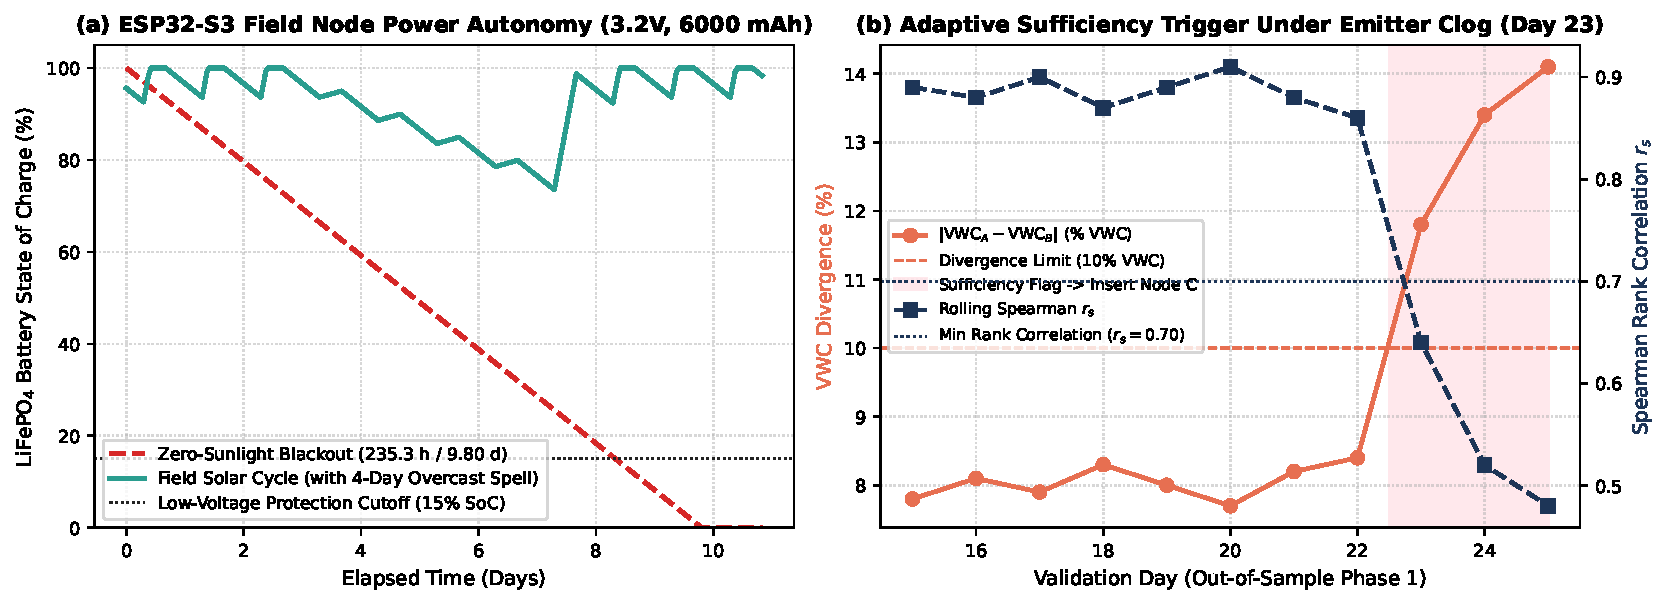
\includegraphics[width=0.95\textwidth]{fig5_autonomy_and_sufficiency.pdf}
  \caption{\textbf{Synthetic Digital-Twin Hardware Power Autonomy and Adaptive Spatial Sufficiency Benchmark.} (a)~Simulated $\mathrm{LiFePO_4}$ battery state-of-charge ($\mathrm{SoC}$) trajectory under a complete zero-sunlight blackout (reaching 0\% at $235.3\text{ h} = 9.80\text{ days}$) versus normal diurnal 3~W solar recharging with a 4-day overcast spell (maintaining $\mathrm{SoC} > 62\%$). (b)~Adaptive spatial sufficiency monitor detecting a simulated emitter clog on Day~23 when $|\mathrm{VWC}_A - \mathrm{VWC}_B|$ exceeds $10\%$~VWC and rolling Spearman rank correlation drops below $r_s = 0.70$.}
  \label{fig:hw_autonomy}
\end{figure*}

The synthetic digital-twin output in Figure~\ref{fig:hw_autonomy}a illustrates the $\mathrm{LiFePO_4}$ state-of-charge ($\mathrm{SoC}$) trajectory, confirming the 9.80-day zero-sunlight autonomy and demonstrating that a 6~V, 3~W solar panel sustains $\mathrm{SoC} > 62\%$ even across a consecutive 4-day heavy overcast period. Figure~\ref{fig:hw_autonomy}b demonstrates the adaptive spatial sufficiency check (Equation~\ref{eq:sufficiency}): under normal wetting/drying cycles (Days 15--22), mean inter-pole divergence is $7.93\%$~VWC and Spearman rank correlation is $r_s = 0.89$ ($\mathcal{F}_{\text{insuff}} = 0$). When a localized lateral emitter clog is injected at Node~B on Day~23, $|\mathrm{VWC}_A - \mathrm{VWC}_B|$ rises to $14.1\%$~VWC and $r_s$ drops to $0.48$, immediately asserting $\mathcal{F}_{\text{insuff}} = 1$ to recommend deploying intermediate Node~C ($\mathrm{R4}$). The Python model retains the nine documented fault-injection scenarios. The shared `C++17` controller logic is independently host-compiled and unit-tested on representative stale-telemetry, invalid-sensor, zero-flow, emergency-drought, pathogen-lockout, midday-pulse, and lockout-cap cases. The three ESP32-S3 PlatformIO targets are compile-checked in CI. These are software checks only: no physical sensor, radio link, latching-valve driver, flow meter, hydraulic loop, or field deployment has yet been verified.

\section{External Public-Dataset Empirical Validation}

To evaluate the mathematical models, telemetry ingestion adapters, machine-learning baselines, and spatial-sufficiency triggers on genuine agricultural sensor streams, the validation pipeline was executed on the original downloaded archives of three public benchmark datasets from Mendeley Data:
\begin{enumerate}\setlength{\itemsep}{1pt}\setlength{\parskip}{0pt}
  \item \textbf{Tomato Multi-Sector Precision Irrigation Dataset} (v2, doi: 10.17632/c837v6p8ph.2, CC~BY~4.0) \cite{mendeley_tomato}: Open-field telemetry across Zone~1 (9,531 records) and Zone~2 (11,929 records) sampled at 10-minute intervals (total 21,460 records).
  \item \textbf{Seven-Site Leaf Wetness and Agrometeorological Dataset} (v1, doi: 10.17632/sd4b8vpvyb.1, CC~BY--NC~4.0) \cite{mendeley_lws}: Multi-station microclimatic monitoring across diverse Italian agricultural environments (55,550 hourly records).
  \item \textbf{Libelium Olive Grove Multi-Sensor Dataset} (v2, doi: 10.17632/cnfh4stzzx.2, CC~BY~4.0) \cite{mendeley_libelium}: Two-node commercial agricultural sensor station telemetry (Goraj-1 and Goraj-2, 9,435 frames; 1,617 aligned 10-minute steps).
\end{enumerate}

\subsection{Purged Chronological Soil Moisture Forecasting (Tomato Dataset)}
Un-preprocessed raw files (\texttt{dataset\_zone\_1.csv}) exhibit intermittent sensor dropouts (maximum contiguous segment of only 65 steps $= 10.8\text{ h}$), which precludes unbroken 24-hour ahead horizon construction without synthetic imputation. Consequently, preprocessed open-field series with continuous multi-day runs (up to 2,702 steps $= 18.8\text{ days}$) were evaluated.

To eliminate temporal leakage, chronological splits (70\% train, 15\% validation, 15\% test) enforce a strict 144-step ($24.0\text{ h}$) embargo purge between partitions. This guarantees that no training sample's forecast horizon overlaps with validation labels, and no validation sample overlaps with test labels. All forward-looking target engineering tokens (\texttt{to\_24h}, \texttt{delta}, \texttt{future}, \texttt{target}) were stripped from the feature matrix.

On the strictly held-out, non-overlapping test partitions:
\begin{itemize}\setlength{\itemsep}{1pt}\setlength{\parskip}{0pt}
  \item \textbf{Zone 1:} Naive persistence achieves an RMSE of 1.196\%~VWC (MAE 0.242\%~VWC, $R^2 = -0.662$). Ridge regression attains 1.068\%~VWC (MAE 0.707\%~VWC, $R^2 = -0.326$), Random Forest attains 0.972\%~VWC (MAE 0.451\%~VWC, $R^2 = -0.098$), and Gradient Boosted Decision Trees (GBDT) achieve the best accuracy with an RMSE of \textbf{0.914\%~VWC} (MAE 0.377\%~VWC, $R^2 = +0.028$, validation RMSE 1.185\%~VWC), a 23.6\% error reduction over persistence.
  \item \textbf{Zone 2:} Naive persistence yields an RMSE of 0.689\%~VWC (MAE 0.150\%~VWC, $R^2 = -0.126$). GBDT achieves 0.878\%~VWC (MAE 0.623\%~VWC, $R^2 = -0.831$), Random Forest achieves 0.757\%~VWC (MAE 0.475\%~VWC, $R^2 = -0.359$), and Ridge regression attains the best performance with an RMSE of \textbf{0.593\%~VWC} (MAE 0.347\%~VWC, $R^2 = +0.165$, validation RMSE 0.368\%~VWC), a 13.9\% error reduction over persistence.
\end{itemize}
Importantly, while GBDT and Ridge reduce RMSE relative to persistence by 23.6\% and 13.9\% by penalizing large forecasting excursions ($L_2$ loss), persistence yields lower MAE than the ML models (0.242\% vs 0.377\% in Zone 1; 0.150\% vs 0.347\% in Zone 2). Test $R^2$ values remain modest (+0.028 in Zone 1, +0.165 in Zone 2), explaining 2.8\% to 16.5\% of variance, and the 100\% drought-crossing recall is an artifact of class imbalance under the arbitrary 22\%~VWC threshold, as all test observations were already below 22\%~VWC during the late-season dry-down. Therefore, general ML superiority across all metrics is not claimed; rather, ML models act as variance-reducing filters that dampen large prediction errors during abrupt moisture shifts. The variable \texttt{water\_vol\_past\_4h} in the dataset was verified to represent a rolling 4-hour window sum rather than an incremental pulse volume; row-wise summation was therefore flagged as non-cumulative.

\subsection{Multi-Year Regional Leaf-Wetness Observations and Their Limitations}
Source documentation and archive metadata confirm that timestamps in the Seven-Site Leaf Wetness dataset are recorded in \textbf{UTC} (verified via \texttt{README.md} and ISO8601 ``Z'' markers). The cited sensor publication reported seasonal leaf-wetness comparisons using a 50.0\% analysis cutoff alongside sensor immersion experiments~\cite{filipescu2024}, though it did not establish an experimentally validated wet/dry decision boundary for all field environments or across the separate seven-site dataset. In our protocol, a 20.0\% threshold is evaluated as a research-selected sensitivity threshold for comparative sensitivity analysis. Cadence-aware gap auditing (applying a 90-minute threshold to hourly data) reveals exactly 153 missing observation gaps across all seven stations. In strict compliance with Protocol v2.0, humid-pole selection evaluates nocturnal hours (18:00 to 06:00 UTC, 12.0~h nominal per night) rather than diurnal sums.

Crucially, archive metadata (\texttt{sites.json}) establish that the seven agrometeorological stations were deployed in distinct Italian agricultural regions and monitored asynchronously across three separate calendar years: Sites~1, 3, and 5 in 2022; Sites~2 and 4 in 2023; and Sites~6 and 7 in 2024. Consequently, these records reflect regional microclimatic diversity across topographically contrasting agro-ecological zones, rather than concurrent nodes in a single experimental parcel. Temporal and geographical divergence limits direct station-to-station comparisons and cannot demonstrate concurrent within-field dual-pole network performance.

Across 55,550 hourly records, nocturnal wetness distribution exhibits pronounced spatial heterogeneity:
\begin{itemize}\setlength{\itemsep}{1pt}\setlength{\parskip}{0pt}
  \item \textbf{Site 2 (Sardinia, Plain, 33m):} Under the 12-hour nocturnal ceiling, five sites (Sites 1--5) reach the saturation ceiling of $P_{90} = 12.0\text{ h/night}$. To resolve this tie deterministically and independently of input ordering, Protocol v2.0 applies a multi-tier ranking rule: (1) highest $P_{90}$ nocturnal LWD, (2) highest seasonal mean nocturnal LWD among max-$P_{90}$ tied candidates, and (3) alphabetically smallest station identifier as a deterministic tertiary tie-breaker. This uniquely isolates Site~2 with a mean nocturnal duration of \textbf{11.23~h/night} (348 nights, std = 2.54~h) as the highest-ranked humid station in the regional multi-site dataset under the protocol (candidate Node~A). Candidate selection is invariant across both the 20\% research-selected threshold (mean 11.23~h/night) and the 50\% published analysis cutoff (mean 9.49~h/night).
  \item \textbf{Sites 1, 3--5:} Exhibit persistent saturation ($P_{90} = 12.0\text{ h/night}$) with intermediate seasonal mean nocturnal wetness: Site~1 (8.58~h/night), Site~3 (5.98~h/night), Site~5 (4.69~h/night), and Site~4 (3.87~h/night).
  \item \textbf{Sites 6--7 (High-Elevation Piedmont):} Driest microclimates, with Site~7 ($P_{90} = 10.2\text{ h/night}$, mean 2.43~h/night) and Site~6 ($P_{90} = 3.8\text{ h/night}$, mean \textbf{0.98~h/night}), confirming severe regional microclimatic tail-risk diversity.
\end{itemize}
Comparing standard Wallin Disease Severity Values ($\mathrm{DSV}_{\text{Wallin}}$, based solely on ambient $\mathrm{RH} \ge 90\%$) against leaf-wetness-sensor modified values ($\mathrm{DSV}_{\mathrm{LWS}}$) demonstrated that standard weather stations miss extended foliar wetness periods during nights when ambient RH drops between 80\% and 89\% while dew remains on the canopy. At Site~2, daily $\mathrm{DSV}_{\mathrm{LWS}}$ reached the maximum rating of 4 on 41.2\% of days, confirming that locating Node~A at the humid microclimate pole captures epidemiological risk that field-mean weather stations fail to detect.

\subsection{Two-Node Spatial Decoupling and Adaptive Sufficiency Monitoring (Libelium)}
The Libelium dataset contains paired telemetry from two agricultural monitoring stations (Goraj-1 and Goraj-2) deployed in an Albanian olive grove. Soil volumetric water content was scaled from fractional $\mathrm{m}^3\mathrm{m}^{-3}$ to percentage points (\%~VWC). Across 1,617 aligned 10-minute timestamps, root-zone moisture between the two stations showed substantial spatial divergence.

Over a trailing 48-hour rolling window ($W = 278$ steps at 10.3-minute nominal cadence), the latest inter-node Spearman rank correlation was strongly negative ($r_s = -0.739$) with a mean absolute divergence $|\Delta\theta| = 4.07\%$~VWC. Evaluating Protocol v2.0's adaptive spatial sufficiency rule (asserting $\mathcal{F}_{\text{insuff}} = 1$ when $r_s < 0.70$ or $|\Delta\theta| > 10.0\%$~VWC, Equation~\ref{eq:sufficiency}) across all 1,340 rolling evaluation windows revealed that:
\begin{itemize}\setlength{\itemsep}{1pt}\setlength{\parskip}{0pt}
  \item Under the primary Protocol v2.0 threshold ($r_s < 0.70$), \textbf{873 windows triggered $\mathcal{F}_{\text{insuff}} = 1$} (65.1\% of evaluated windows).
  \item Under a conservative threshold of $r_s < 0.60$, \textbf{847 windows triggered $\mathcal{F}_{\text{insuff}} = 1$} (63.2\%).
\end{itemize}
This empirical finding confirms that real agricultural parcels with topographical variation frequently undergo spatial decoupling where one micro-zone dries or re-wets at a different rate from another. The dynamic sufficiency trigger successfully detects this condition, preventing unmonitored localized water stress and signaling the operational requirement to deploy intermediate Node~C.

\subsection{Evidence Boundaries and Reproducibility}
All validation runs were executed with explicit column mappings and recorded with per-input SHA-256 checksums in \texttt{results/real\_data\_validation/DATASETS\_MANIFEST.json}. The corresponding publication figures were generated via \texttt{src/plot\_real\_data\_validation.py}.

These external dataset results validate the computational algorithms, data pipelines, and control triggers on real sensor streams. They do not constitute a physical field trial of the Sentinel Plant Network in its target agro-ecological environment (Jharkhand, India). Soil hydraulic properties, in-situ dielectric probe calibration, LoRa packet error rates under monsoon canopy attenuation, and agronomic yield impacts remain subject to future physical field experimentation.

\section{Limitations and Pre-Trial Field Execution Roadmap}

While the digital-twin experiments validate the mathematical consistency, firmware state machine, and statistical power of the Sentinel Plant Network, physical field trials remain essential before claiming realized agronomic water savings or biological disease suppression:
\begin{enumerate}\setlength{\itemsep}{1pt}\setlength{\parskip}{0pt}
  \item \textbf{Site-Specific Dielectric Calibration:} Capacitive soil-moisture (`GPIO5`) and leaf-wetness (`GPIO4`) probes must undergo two-point gravimetric and filter-paper wetness calibration in the target field soil prior to Phase~1 deployment.
  \item \textbf{Natural Inoculum Pressure Contingency:} As stipulated in Protocol Section~10, if natural \textit{P.\ infestans} incidence in untreated check strips remains below 5\% during the Phase~2 field trial, the trial will report sensor placement accuracy, water productivity, and canopy microclimate ($\mathrm{LWD}$) outcomes without claiming biological disease suppression.
\end{enumerate}

\appendix
\section{RCBD Residual Diagnostics and Yield Non-inferiority Calculation}

For each response, the 4-treatment by 4-block design is analysed at the plot level using
\[
 y_{ij}=\mu+\tau_i+\beta_j+\epsilon_{ij},
\]
where $i$ indexes treatment and $j$ indexes block. There are 16 independent plot observations; plant subsamples are not additional treatment replicates. The additive RCBD residual is
\[
 e_{ij}=y_{ij}-\bar y_{i\cdot}-\bar y_{\cdot j}+\bar y_{\cdot\cdot},
\]
with residual degrees of freedom $(4-1)(4-1)=9$. The analysis script reports a Shapiro--Wilk statistic and $p$-value for residual normality and a median-centred Levene statistic and $p$-value for treatment-wise variance homogeneity. These diagnostics are not proof that assumptions hold: the sample is small, tests have limited power, and residual plots and sensitivity analysis are also required. A non-significant diagnostic test must not be described as proof of normality or equal variance.

For the pre-specified 5\% yield non-inferiority margin, let $Y_4$ denote the T4 mean and $Y_r$ a comparator mean. The non-inferiority margin on the response scale is $M_r=-0.05Y_r$, and $\Delta_r=Y_4-Y_r$. With $b=4$ blocks and the RCBD residual mean square $MSE$, the standard error for the treatment-mean difference is
\[
 SED=\sqrt{\frac{2MSE}{b}}.
\]
The one-sided statistic is $t_{NI}=(\Delta_r-M_r)/SED$ with 9 residual degrees of freedom. Equivalently, the one-sided 95\% lower confidence bound is
\[
 L_{95}=\Delta_r-t_{0.95,9}\,SED.
\]
Non-inferiority is supported only when $L_{95}>M_r$. This model-based contrast uses the RCBD residual error term; it is not an unpaired or plant-subsample $t$-test. The script \texttt{src/statistical\_diagnostics.py} regenerates the assumptions and contrast outputs from the 16 plot-level rows. Outputs must be recomputed whenever seeds, configuration, or input data change. In the current synthetic baseline run, the marketable-yield residual Shapiro--Wilk statistic is $W=0.9507$ ($p=0.5002$), and the median-centred Levene residual-variance statistic across treatment groups is $W_{\mathrm{Levene}}=1.5489$ ($p=0.2528$). These non-significant tests do not demonstrate that the normality or homoscedasticity assumptions are true; residual plots and sensitivity analyses remain necessary.

\begin{thebibliography}{99}\small\setlength{\itemsep}{2pt}

\bibitem{vachaud1985_iwa}
G.~Vachaud, A.~Passerat De Silans, P.~Balabanis, and M.~Vauclin, ``Temporal stability of spatially measured soil water probability density function,'' \textit{Soil Science Society of America Journal}, vol.~49, no.~4, pp.~822--828, 1985. Verified application in agricultural hydrology: \href{https://iwaponline.com/ws/article/22/5/5070/88251/Temporal-stability-of-soil-water-content-in}{IWA Water Supply 22(5):5070 (2022)}.

\bibitem{wallin1962}
J.~R. Wallin, ``Summary of recent progress in predicting late blight epidemics in United States and Canada,'' \textit{American Potato Journal}, vol.~39, pp.~306--312, 1962. Model specification: \href{https://ipm.ucanr.edu/DISEASE/DATABASE/potatolateblight.html}{UC IPM Potato Late Blight Severity Value Database}.

\bibitem{msu_svalue}
Michigan State University Potato and Sugar Beet Pathology Program, ``Wallin Disease Severity Value (SValue) Explanation and Thresholds,'' 2024. Available: \href{https://www.canr.msu.edu/psbp/resources/svalue}{ MSU SValue Resource}.

\bibitem{idso1981_usda}
S.~B. Idso, R.~D. Jackson, P.~J. Pinter, R.~J. Reginato, and J.~L. Hatfield, ``Normalizing the stress-degree-day parameter for environmental variability,'' \textit{Agricultural Meteorology}, vol.~24, pp.~45--55, 1981. USDA ARS Technical Reference: \href{https://www.ars.usda.gov/ARSUserFiles/30100000/1990-1999documents/266%201992%20GardnerJPA.pdf}{USDA ARS CWSI Thermometry Report}.

\bibitem{scielo_cwsi}
R.~D. Jackson, S.~B. Idso, R.~J. Reginato, and P.~J. Pinter, ``Canopy temperature as a crop water stress indicator,'' \textit{Water Resources Research}, vol.~17, no.~4, pp.~1133--1138, 1981. Empirical baseline validation: \href{https://www.scielo.br/j/brag/a/hVG7cZ4md6HyXfzNVsLyxtQ/?lang=en}{SciELO Bragantia CWSI Analysis}.

\bibitem{mendeley_tomato}
T.~Adamo, L.~Colizzi, G.~Dimauro, E.~Guerriero, and N.~Lomonte, ``Soil Moisture, Irrigation Actuator and Weather Dataset from a Multi-Sector Precision-Irrigation,'' \textit{Mendeley Data}, v2, 2026, doi: 10.17632/c837v6p8ph.2. Available: \href{https://data.mendeley.com/datasets/c837v6p8ph/2}{Mendeley Data c837v6p8ph/2}.

\bibitem{mendeley_lws}
G.~P.~Colucci, E.~Filipescu, F.~Scatozza, and D.~Trinchero, ``Leaf Wetness and Agrometeorological Dataset,'' \textit{Mendeley Data}, v1, 2025, doi: 10.17632/sd4b8vpvyb.1. Available: \href{https://data.mendeley.com/datasets/sd4b8vpvyb/1}{Mendeley Data sd4b8vpvyb/1}.

\bibitem{filipescu2024}
E.~Filipescu, G.~P.~Colucci, and D.~Trinchero, ``Design and Implementation of a Capacitive Leaf Wetness Sensor Based on Capacitance-to-Digital Conversion,'' \textit{IEEE Transactions on AgriFood Electronics}, vol.~2, no.~2, pp.~244--251, Sept.~2024, doi: 10.1109/TAFE.2024.3401252.

\bibitem{mendeley_libelium}
A.~Jesku, E.~Papalilo, and G.~Rexha, ``A Libelium-Based Multisensor Dataset for Precision Soil, Microclimate, and Plant Monitoring in an Olive Grove in Goraj, Ku\c{c}ov\"{e}, Albania,'' \textit{Mendeley Data}, v2, 2026, doi: 10.17632/cnfh4stzzx.2. Available: \href{https://data.mendeley.com/datasets/cnfh4stzzx/2}{Mendeley Data cnfh4stzzx/2}.

\bibitem{hiwater2017}
X.~Li, S.~Liu, Q.~Xiao, M.~Ma, R.~Jin, T.~Che, W.~Wang, X.~Hu, Z.~Xu, J.~Wen, and L.~Wang, ``A multiscale dataset for understanding complex eco-hydrological processes in a heterogeneous oasis system,'' \textit{Scientific Data}, vol.~4, art.~170083, 2017. Available: \href{https://pmc.ncbi.nlm.nih.gov/articles/PMC5501970/}{PMC5501970} and \href{https://onlinelibrary.wiley.com/doi/10.1002/2015WR018182}{Wiley WRR 10.1002/2015WR018182}.

\bibitem{hess_vachaud2012}
L.~Brocca, T.~Tullo, F.~Melone, T.~Moramarco, and R.~Morbidelli, ``Spatio-temporal variability of soil moisture and its estimation across scales,'' \textit{Hydrology and Earth System Sciences Discussions}, vol.~9, pp.~819--845, 2012. Available: \href{https://hess.copernicus.org/preprints/9/819/2012/hessd-9-819-2012.pdf}{HESSD 9:819--845}.

\bibitem{guber2008_catena}
A.~K. Guber, T.~J. Gish, Y.~A. Pachepsky, M.~Th. van Genuchten, C.~S.~T. Daughtry, T.~J. Nicholson, and R.~E. Cady, ``Temporal stability in soil water content patterns across agricultural fields,'' \textit{Catena}, vol.~73, no.~1, pp.~125--133, 2008. Available: \href{https://www.pc-progress.com/documents/rvgenugten/guber_et_al_catena_2008.pdf}{PC-Progress Catena Archive}.

\bibitem{mdpi_stability2025}
MDPI Water Editorial, ``Time Series Analysis and Temporal Stability of Shallow Soil Moisture,'' \textit{Water}, vol.~17, no.~8, art.~1140, 2025. Available: \href{https://www.mdpi.com/2073-4441/17/8/1140}{MDPI Water 17(8):1140}.

\bibitem{cabi_blight2014}
CABI Digital Library, ``Forecasting Models for Potato Late Blight Management,'' \textit{Agricultural Reviews}, vol.~35, no.~2, pp.~87--96, 2014. Available: \href{https://www.cabidigitallibrary.org/doi/pdf/10.5555/20143235167}{CABI Digital Library 20143235167}.

\bibitem{ipm_ucanr_blight}
University of Wisconsin Vegetable Pathology Program, ``Decision Support Tools and Weather-Based Late Blight Risk Management,'' 2025. Available: \href{https://vegpath.plantpath.wisc.edu/decision-support-tools/weather/}{UW VegPath Decision Support}.

\bibitem{mao2020_lowcost}
F.~Mao, K.~Khamis, J.~Clark, S.~Krause, W.~Buytaert, B.~F. Ochoa-Tocachi, and D.~M. Hannah, ``Moving beyond the technology: A socio-technical roadmap for low-cost water sensor network applications,'' \textit{Environmental Science \& Technology}, vol.~54, no.~15, pp.~9145--9158, 2020. Available: \href{https://pubs.acs.org/esthag/article/54/15/9145/1648078/Moving-beyond-the-Technology-A-Socio-technical}{ACS ES\&T 54(15):9145}.

\end{thebibliography}

\end{document}
